\section{Results}\label{sec:results}

\subsection{Complete grounding}

Every one of the 106 clauses of the Specification carries at least one recorded ground, and every one of the 79 adopted forms is cited by at least one clause. The 183 grounding edges close both directions, so no clause stands without a stated basis and no adopted form was collected and then left unused. Completeness in this sense is a property of the record and not of the argument: an edge states that a clause was written from that ground, and no check grades how well the clause serves it.

The grounds are not of one kind. Of the 183 edges, 135 reach an adopted form, 41 reach a frozen principle, 6 reach a goal unit, and 1 reaches a goal section. 96 of the 106 clauses name at least one adopted form, and the remaining 10 rest on a principle or on a stated goal alone. To call the layer a clause-to-pattern mapping would hide those 10 clauses, which are the ones whose basis is the project's own objective rather than collected practice.

The load is uneven on both sides. 64 clauses cite one ground, 31 cite two, 7 cite three, 3 cite four, and clause \hyperlink{nss-16.2}{16.2} cites 24, because it lists the mandatory checks and inherits the grounds of everything it checks. 45 of the 79 adopted forms are cited by one clause, 20 by two, 11 by three, 1 by five, and 2 by six. The clauses that cite a given adopted form are listed by a query over the grounding edges.

Table~\ref{tab:corpus} states the measured sizes of the corpus and its derived layers. Every count in it was recomputed on 2026-09-21 against the dependency database named in Appendix~\ref{app:repro}, opened read-only, and none was copied from an earlier working note.

\begin{table*}[t]
\centering
\caption{Measured properties of the corpus and its derived layers, recomputed 2026-09-21 against the fixed dependency database described in Appendix~\ref{app:repro}. The semantic relations are delegated-AI single-lane output under the review conditions described in Appendix~\ref{app:repro}, and are neither human ratification nor dual-lane consensus.}
\label{tab:corpus}
\begin{tabular}{p{2.1in}p{0.8in}p{3.5in}}
\toprule
Property & Count & Basis \\
\midrule
Source nodes & 3{,}853 & Deterministic parse of the four documents into a containment tree \\
\addlinespace
Nodes in total & 4{,}206 & Source nodes plus 353 ratified semantic symbols \\
\addlinespace
Directed edges & 8{,}913 & Eleven edge types, structural and semantic together \\
\addlinespace
Clauses, and clauses grounded & 106, 106 & Outbound grounding links per clause \\
\addlinespace
Adopted forms, and forms cited & 79, 79 & Inbound grounding links per adopted form \\
\addlinespace
Grounding edges & 183 & 135 to an adopted form, 41 to a principle, 7 to the goal document \\
\addlinespace
Requirement units & 572 & One sentence each, addressed by document and byte range \\
\addlinespace
Units compiled, and classified gaps & 360, 212 & Extraction status recorded per unit \\
\addlinespace
Propositions & 544 & Validated rule records from the 360 compiled units \\
\addlinespace
Clause-to-goal links & 331 & Reviewed clause-to-goal pass, 2{,}332 recorded decisions \\
\addlinespace
Clauses linked to a goal, goal units linked & 81 of 106, 17 of 22 & Distinct endpoints of the clause-to-goal links \\
\addlinespace
Dependency links & 157 & Tiled dependency pass with blind review and adjudication \\
\addlinespace
Semantic symbols, and symbols carrying an edge & 353, 151 & Ratified registry, and endpoint membership in the edge set \\
\bottomrule
\end{tabular}
\end{table*}

\subsection{Requirement representation and missing goal paths}

The corpus divides into 572 requirement units, of which 360 compiled into 544 validated propositions and 212 produced a classified gap. Figure~\ref{fig:coverage} shows the split and the composition of the gap set. A gap is a recorded refusal rather than a silent omission: each one names the unit, its byte range, the reason it could not be represented, and the remediation it would need.

\begin{figure*}[t]
\centering
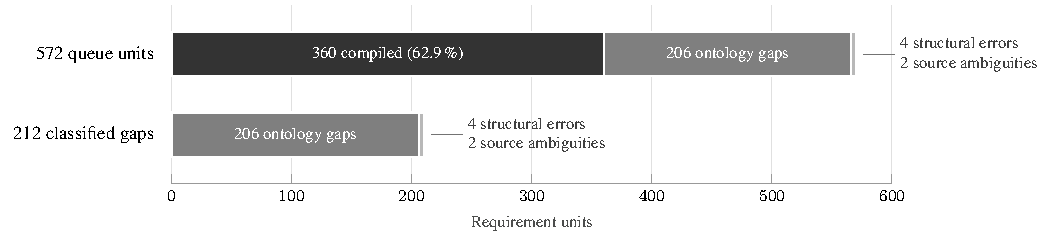
\includegraphics[width=\textwidth]{figures/f08/f08-coverage.pdf}
\caption{Representation coverage over the 572 requirement units. 360 units compiled into propositions and 212 were recorded as classified gaps, of which 206 are ontology gaps, 4 are structural errors, and 2 are source ambiguities. The abstention is explicit and addressable: each gap carries its unit, its byte range, and its required remediation.}
\label{fig:coverage}
\end{figure*}

Of the 212 gaps, 206 are ontology gaps, where the sentence names a concept the controlled vocabulary does not carry, 4 are structural errors, and 2 are source ambiguities. The gap population is therefore dominated by vocabulary coverage rather than structural failure or source ambiguity.

The modality field is concentrated in obligation. 432 of the 544 propositions are required actions, 85 are prohibited actions, 25 are permitted actions, and 2 are definitional, so 517 state an action that is required or forbidden and 27 do not.

The actor field is concentrated further. 504 of the 544 propositions bind the generic project actor, 13 bind an executor, 11 a human authority, 10 an AI agent, 2 a named human owner, 2 a declared role, and 2 carry no actor. The authority-leakage check exists to find an obligation placed on the wrong party, and on this corpus it has at most 40 propositions to rule on even after the authority matrix is populated.

Goal paths were built as a separate reviewed pass. 331 clause-to-goal links were retained from 2{,}332 recorded clause-and-goal decisions, under the named single-lane relation policy with delegated-AI ratification. Those edges are not human ratification and not dual-lane consensus, and the second lane over this pass is open by decision rather than by oversight.

81 of the 106 clauses reach at least one goal unit, and 25 reach none. A covered clause carries between 1 and 11 edges with a mean of 4.09, and a covered goal unit receives between 1 and 36 with a mean of 19.47. Figure~\ref{fig:relation-graph} shows the distribution of the edges by clause section and goal band.

\begin{figure}[t]
\centering
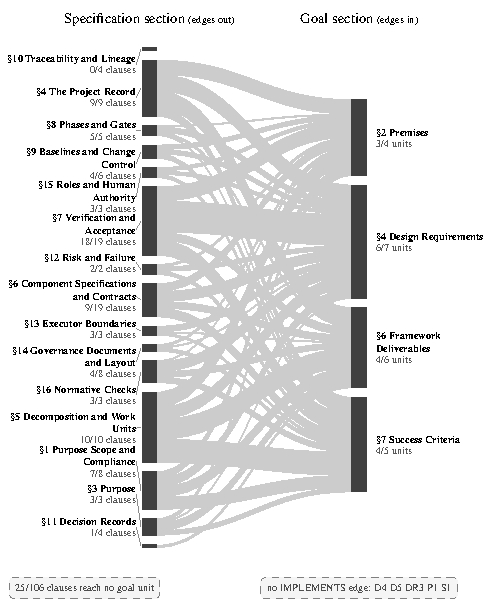
\includegraphics[width=\columnwidth]{figures/f09/f09-relation-graph.pdf}
\caption{The reviewed clause-to-goal relation, aggregated from 331 clause-to-goal links into bands between clause sections on the left and goal units on the right, with band thickness proportional to edge count. The edges are delegated-AI single-lane output under the production review conditions in Appendix~\ref{app:repro}. 25 of the 106 clauses appear on no band because no path to a stated goal was recorded for them.}
\label{fig:relation-graph}
\end{figure}

The 25 unlinked clauses are not scattered through the document. They are all four clauses of the traceability section, ten clauses of the component-specification section, four of the governance-document section, three of the decision-record section, and clauses \hyperlink{nss-1.4}{1.4}, \hyperlink{nss-7.10}{7.10}, \hyperlink{nss-9.5}{9.5}, and \hyperlink{nss-9.6}{9.6}. Most govern how the project record is organised, labelled, linked, or kept consistent, rather than what the engineered system must do.

The reverse direction is sparse for a different reason. 17 of the 22 goal units receive at least one inbound edge and 5 receive none. Two of the five are deliverables the project has not built, two are the requirement and the acceptance criterion for that unbuilt work, and one is a premise, which nothing should implement by kind.

Three readings of the 25 survive the evidence, and the record does not choose between them. The Specification may carry record-keeping machinery that no stated objective asked for. The goal document may be under-specified, so that real objectives exist but were never written as goal units. Or one review lane may have missed links that a second lane would find. A second lane restricted to those 25 clauses separates the third reading from the first two, and no cheaper evidence does.

\subsection{Dependency structure and graph size}

The dependency pass evaluated 42{,}400 ordered candidate cells and proposed 240 edges; the retained graph holds 157. 75 of the pass's 240 answers were overturned in review, so reading the pass output as the graph would have been wrong by roughly a third. Every retained edge carries at least two separate judgments: 127 carry two, 23 carry three, and 7 carry four. 131 were settled by a blind reviewer who agreed with the pass without seeing it, 11 at a third round, 7 at a second, 5 by adjudication, 2 by a final ruling, and 1 by an audit of the negatives.

The edges touch less of the corpus than their number suggests. 126 of the 212 possible endpoints appear in the graph, 85 as the source of an edge and 72 as its target. So a change to a clause outside that set has no recorded dependent, which is a statement about the pass and its scope and not a guarantee that nothing depends on the clause.

Four directed cycles were retained by decision rather than removed. Two adopted forms depend on each other, clauses \hyperlink{nss-9.1}{9.1} and \hyperlink{nss-9.2}{9.2} depend on each other, and two longer rings close through clauses \hyperlink{nss-9.3}{9.3} and \hyperlink{nss-9.5}{9.5}. A ruling judged each ring as a ring and kept it, because the baseline and change-control clauses genuinely define one another. These cycles are in the Specification's own semantic graph. They are not a violation of the rule that a project's component graph must be acyclic, which binds a project's decomposition and not a description of the document.

Figure~\ref{fig:dependency-structure} reduces the 103 clause-to-clause edges to relations between sections. The section order along both axes is computed by an exact minimum-backward-weight search over the inter-section weights, so the 8 backward edges that remain are a property of the data rather than of the section numbering or my choice of axis order. The reduction exposes roles that the edge list alone does not show: the normative-checks section sends 15 dependencies and receives none, the decision-record section receives 13 and sends 1, and the terminology and traceability sections neither send nor receive.

\begin{figure*}[tp]
\centering
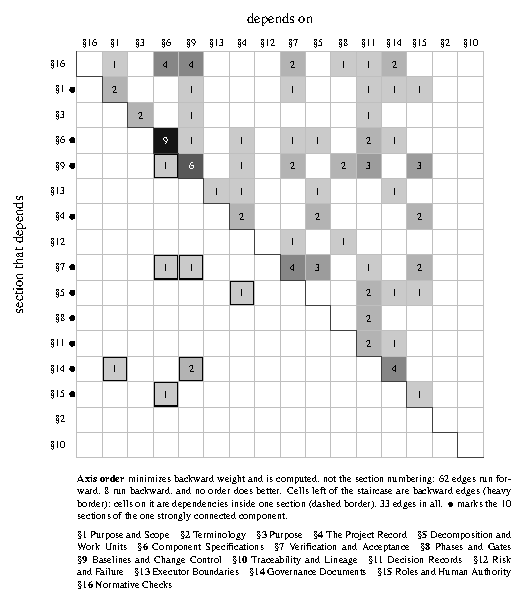
\includegraphics[width=\textwidth]{figures/f10/f10-dependency-structure.pdf}
\caption{The 103 clause-to-clause dependency links aggregated into an ordered section matrix, with 62 edges forward of the diagonal, 33 within a section, and 8 backward. The axis order minimises backward weight exactly, so the backward count measures the corpus and not the section numbering. The dependency links were produced by one model lane, then reviewed and adjudicated under delegated AI authority, with no human verification recorded on any edge.}
\label{fig:dependency-structure}
\end{figure*}

The whole graph holds 4{,}206 nodes and 8{,}913 directed edges across eleven types, drawn in Figure~\ref{fig:semantic-graph} as 8{,}905 undirected lines after eight parallel pairs collapse. 151 of the 353 semantic symbols carry an edge and 202 do not. The 202 resolve into 157 actions that the schema stores as a proposition field rather than as an edge, and 45 further ratified symbols that no proposition refers to. The worked change of Section~\ref{sec:checks} traverses this graph and marks 762 of the 3{,}853 source nodes as possibly affected.

\subsection{Corrections, clashes, and replay}

Verification of the final dependency database returns a pass with an exit code of zero over seventeen checks. Five checks report findings: 25 clauses with no outbound goal link and 5 goal units with no inbound one, at warning severity, 4 directed cycles at warning severity, 39 deontic clashes at informational severity under a recorded ruling, and the 212 extraction gaps at informational severity. Twelve checks report nothing, including database and foreign-key integrity, dangling endpoints, duplicate relation edges, relation provenance, and the validity of all 544 rule records.

The 39 clashes are the one finding class that a ruling moved. Each is a pair in which one proposition requires an action and another forbids it for the same actor and target. The ruling of 2026-09-17 records that every one of the 39 is raised by a restrictive prescription whose restricting complement the rule schema has no slot to hold. The pair is therefore an artifact of the representation and not one of 39 contradictions in the prose. The ruling lowers the severity to informational and leaves all 39 findings visible, and it does not assert that the clauses agree; it asserts that the schema cannot yet tell a conditional prohibition from an absolute one. The remedy it names is a schema slot, and until that slot exists the finding stays in the output.

The deterministic text checks hold 24 warnings in the final dependency database: 19 uses of a defined term in lower case, 4 capitalized phrases that no definition covers, and 1 defined term that nothing refers to. One finding of error severity was detected and repaired before this database was built. The hand-maintained coverage list in \hyperlink{nss-appB}{Appendix~B} of the Specification claimed five clauses for one principle where the generated list holds six, having omitted clause \hyperlink{nss-1.8}{1.8}. The source was corrected on 2026-09-17, and the finding is absent from the final dependency database while it remains in the two earlier ones.

Table~\ref{tab:findings} collects the findings of the whole programme with the procedure that detected each one and the action it produced. The construction findings of Section~\ref{sec:method} are carried in it, because a correction made during construction and a finding retained in the final analysis are both dispositions of the same record.

\begin{table*}[t]
\centering
\caption{Findings, dispositions, and the action each one produced. Graph findings were recomputed on 2026-09-21 against the final dependency database; construction counts are those of Table~\ref{tab:stages}.}
\label{tab:findings}
\begin{tabular}{p{1.05in}p{0.6in}p{1.6in}p{1.5in}p{1.42in}}
\toprule
Finding & Count & Detection procedure & Decision or correction & Resulting action \\
\midrule
Adopted forms needing revision & 21 of 79 & Isolated verification pass, three tests per form & Revised, then rechecked by a third model & Terminology set grew from 13 to 21 terms \\
\addlinespace
Rejected statements readmitted & 5 of 106 & Secondary rule on the recorded rejection reason & Readmitted, each with a written justification & 118 candidates entered generalization \\
\addlinespace
Support ratings on evidence & withdrawn & Evidence audit of the rating instrument & Ratings discarded after review and failed controls & No support rating is reported \\
\addlinespace
Coverage list omits a clause & 1 error & Comparison of the generated and written coverage lists & Source corrected 2026-09-17 & Finding absent from the final dependency database \\
\addlinespace
Deontic clashes & 39 & Conflict check over the 544 propositions & My ruling of 2026-09-17: one schema artifact & Severity lowered to informational, all 39 stay visible; schema slot required \\
\addlinespace
Clauses with no goal path & 25 of 106 & Clause-to-goal coverage check & Retained, unresolved & A second lane over the 25 is the next evidence \\
\addlinespace
Goal units with no inbound link & 5 of 22 & Inbound goal-link check & Retained; four cover unbuilt work, one is a premise & No change to the Specification \\
\addlinespace
Directed cycles & 4 & Cycle detection over recorded dependencies & Each ring judged as a ring and kept & Retained at warning severity \\
\addlinespace
Units with no proposition & 212 of 572 & Extraction gap queue, one entry per unit & Classified, each with its required remediation & 206 are vocabulary work on a known queue \\
\addlinespace
Terminology warnings & 24 & Lower-case use, undefined phrase, unreferenced definition & Retained as warnings & Retained in the analysis record \\
\bottomrule
\end{tabular}
\end{table*}

The internal rebuild test reproduced the relation graph exactly from its recorded decisions. The rebuilt graph had the same logical fingerprint as the original, and the two database files were byte-identical. A separate check recomputed the dependency database's fingerprint and confirmed its recorded value. Repeated derived exports were also byte-identical. The relation graph was rebuilt; the dependency database was not. These checks did not repeat the model calls behind the recorded decisions.

Replay settles reproduction and not acceptance. A rebuilt fingerprint shows that the same inputs and the same decisions give the same graph, and it says nothing about whether the purpose is the right purpose or the residual risk is tolerable. Those remain human decisions, and the record exists so that a person makes them against stated evidence rather than against a recollection.

The four source documents on disk have changed since the graph was frozen. A terminology rename on 2026-09-21 altered 24 requirement units across the four files. The change-detection command reports 507 seed nodes, no parse error, no new finding, and one finding resolved, and the digest table accepts the new bytes as terminology-only successors to the frozen ones. Every count reported above is therefore stated against the named frozen artifacts, whose digests are recorded, and not against the working copy.

Appendix~\ref{app:repro} binds the measurements to their input stages, counting rules, and review conditions. The internal rebuild checks establish repeatability from retained inputs and decisions. They do not establish independent reproduction or agreement between new model judgments.
